% !TeX spellcheck = de_DE
\section{Neuronale Netze}
Klassische Algorithmen in der Informatik beschreiben mit welchen Schritten ein spezielles Problem gelöst werden kann. In vielen Anwendungsfällen, wie zum Beispiel beim Sortieren einer Liste, verwenden Computersysteme diese und lösen das gegebene Problem schneller und effizienter als es Menschen möglich ist. 

Dennoch gibt es Aufgaben, die von Menschen ohne Aufwand gelöst werden, aber Computersysteme vor große Herausforderungen stellen. Hierzu zählt unter anderem die Klassifizierung von Bildern. Ein Mensch kann Bilder von Hunden und Katzen unabhängig von Blickwinkel und Bildqualität unterscheiden beziehungsweise richtig zuordnen. Trotzdem lassen sich für solche Probleme keine klassischen Algorithmen finden, da die Lösung von vielen subtilen Faktoren abhängt \cite{kriesel2008kleiner}.

In vielen dieser Aufgabenfelder werden \ac{KNN} eingesetzt, welche von den biologischen neuronalen Netzen inspiriert sind und zum Forschungsgebiet des maschinellen Lernens gehören. Die Grundlage für die \ac{KNN} bildet die Arbeit von \citeauthor{mcculloch1943logical}, in der sie 1943 ein einfaches neuronales Netz mit Schwellwerten entwickelt haben. Dies ermöglicht die Berechnung von logischen und arithmetischen Funktionen \cite{mcculloch1943logical}. In den folgenden Jahrzehnten wird die Funktionsweise der neuronalen Netze weiterentwickelt und der Einsatz in verschiedensten Aufgabenfeldern ermöglicht. Hierzu zählen neben der Klassifizierung von Bildern \cite{krizhevsky2012imagenet} unter anderem das Erkennen und die Interpretation von Sprache \cite{hinton2012deep}, \cite{andor2016globally} sowie das selbständiges Lösen von Computer- und Gesellschaftsspielen \cite{mnih2013playing}, \cite{silver2016mastering}. 

In diesem Kapitel wird zuerst ...
\subsection{Biologische neuronale Netze}
\label{subsec:biological_neuraL_networks}
Wie bereits beschrieben orientiert sich das Fachgebiet der \ac{KNN} an den erfolgreichen biologischen neuronalen Netzen, wie zum Beispiel dem menschlichen Gehirn \cite{kriesel2008kleiner}. In diesem Abschnitt werden die Eigenschaften betrachtet, die das Vorbild erfolgreich machen und für die \ac{KNN} übernommen werden sollen. Im Zuge dessen wird ein grober Überblick über die Struktur und Funktionsweise des menschlichen Gehirns gegeben. 
\\\\
Jede Sekunde erfassen die Rezeptoren des menschlichen Körpers unzählige Reize, wie zum Beispiel Licht, Druck, Temperatur und Töne. Die Reize werden anschließend elektrisch oder chemisch kodiert und über Nervenbahnen an das Gehirn geleitet, welches die Aufgabe hat diese zu filtern, zu verarbeiten und entsprechend zu reagieren. Als Reaktion können zum Beispiel Signale an entsprechende Muskeln oder Drüsen gesendet werden \cite{kinnebrock2018neuronale}. 

Bevor im nächsten Kapitel die Funktionsweise des Gehirns näher betrachtet wird, sollen drei Eigenschaften genannt werden, die klassische Algorithmen nicht besitzen beziehungsweise nur schwer umsetzen können, aber für biologische neuronale Netze keine Herausforderung sind. Ziel ist es, diese für die \ac{KNN} zu übernehmen \cite{kriesel2008kleiner}.
\begin{enumerate}
	\item \textbf{ Fähigkeit zu Lernen} \\
	Das menschliche Gehirn ist nicht wie ein klassischer Algorithmus für seine Aufgaben programmiert. Stattdessen besitzt es die Fähigkeit anhand von gegebenen Beispielen und oder einfachem Ausprobieren zu lernen \cite{kriesel2008kleiner}. Hierbei wird das gewünschte Ergebnis mit dem tatsächlich erhaltenen Ergebnis verglichen und das Verhalten entsprechend angepasst. Dies ermöglicht es Menschen verschiedenste Aufgabengebiete erfolgreich zu lösen und sich ändernden Anforderungen anzupassen.
	
	\item \textbf{Fähigkeit zur Generalisierung}\\
	Allerdings kann nicht jedes mögliche Szenario für ein Aufgabenfeld durch Ausprobieren oder Beobachtung gelernt werden. Trotzdem trifft das Gehirn in den meisten Situationen plausible Lösungen, da es die Fähigkeit zur Generalisierung besitzt 
	\cite{kriesel2008kleiner}. Das bedeutet, dass viele Situationen bereits bekannten Problemen zugeordnet werden können, mithilfe derer eine passende Verhaltensstrategie ausgewählt wird. 
	
	\item \textbf{Toleranz gegenüber Fehlern}\\
	Die Fähigkeit zu Generalisieren erlaubt auch eine hohe Fehlertoleranz gegenüber verrauschten Daten. Bei dem oben genannten Beispiel der Klassifizierung von Bildern kann ein Teil des Bildes fehlen oder unscharf sein und trotzdem kann das abgebildete Motiv richtig zugeordnet werden.
\end{enumerate}

\subsubsection{Struktur des menschlichen Gehirns}
Die Forschungsgebiet der Neurowissenschaften befasst sich unter anderem mit dem menschlichen Gehirn, dessen Funktionsweise noch nicht vollständig nachvollzogen werden kann. Trotzdem ist schon seit 1861 durch die Arbeit von Paul Broca bekannt, dass es im menschlichen Gehirn verschiedene Regionen mit unterschiedlichen Aufgaben gibt \cite{russell2013kunstliche}. Zum Beispiel wird das sogenannte Kleinhirn (Cerebellum) für einen Großteil der motorischen Koordination verwendet während an das Großhirn (Telencephalon) unter anderem visuelle Reize geleitet werden \cite{kriesel2008kleiner}. Trotz der unterschiedlichen Aufgaben haben alle Bereiche des Gehirns einen gemeinsamen Grundbaustein, die sogenannten Neuronen \cite{russell2013kunstliche}. Im folgenden wird der Aufbau und die Funktionsweise von diesen oberflächlich im Bezug zu den später vorgestellten künstlichen Neuronen betrachtet. Für einen vollständigen Überblick und eine genaue Beschreibung der Vorgänge wird auf entsprechende Fachliteratur verwiesen.\\
%TODO Fachliteratur LINK
\begin{figure}[h]
	\centering
	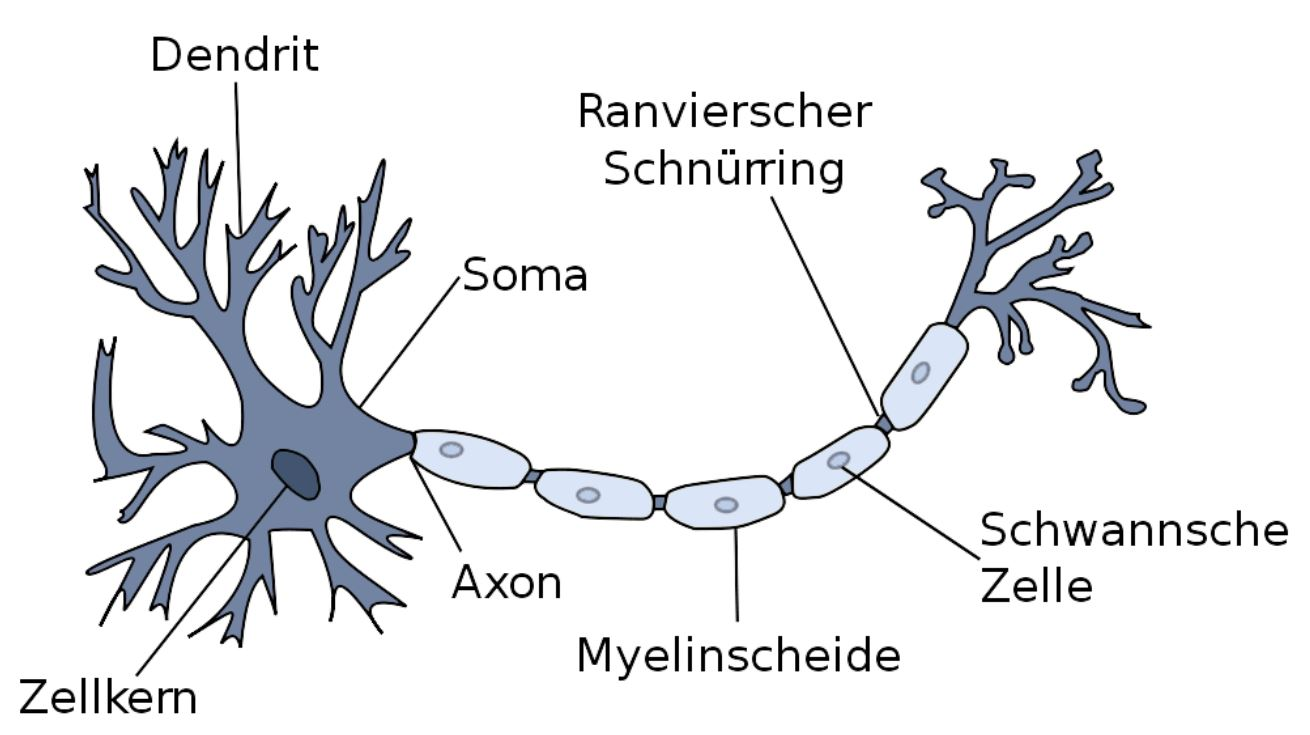
\includegraphics[width=0.75\textwidth]{./img/biologial_neuron.JPG} 
	\caption{Schematische Abbildung einer Nervenzelle, Quelle \cite{kriesel2008kleiner}.}
	\label{fig:biological_neuron}
\end{figure}
Das menschliche Gehirn besitzt ungefähr ${10}^{11}$ einzelne Neuronen, deren schematischer Aufbau in \autoref{fig:biological_neuron} dargestellt ist. Jedes Neuron besitzt einen Zellkern, der sich im Zellkörper (Soma) befindet. Von dem Zellkörper gehen mehrere Fasern aus, die Dendriten genannt werden \cite{russell2013kunstliche}. An diesen befinden sich Synapsen, welche als Übertragungsstelle fungieren und elektrische oder chemische Signale von Rezeptoren oder anderen Neuronen empfangen \cite{kriesel2008kleiner}. Typischerweise empfängt ein Neuron Signale von 2000 und 10.000 anderen Nervenzellen \cite{zell2003simulation}. \\
Synapsen, die elektrische Signale empfangen, haben eine starke, direkte, nicht regulierbare Verbindung vom Sender zum Empfänger. Diese sind für hart kodierte Verhaltensmechanismen nützlich wie zum Beispiel den Fluchtreflex. Die chemische Synapse hingegen ist nicht direkt mit dem Sender verbunden, sondern durch den synaptischen Spalt getrennt \cite{kriesel2008kleiner}. Zur Übertragung eines elektrischen Signals wird dieses auf der präsynaptischen Seite in ein chemisches Signal kodiert, indem Neutransmitter freigesetzt werden. Diese können über den synaptischen Spalt übertragen und anschließend auf der postsynaptischen Seite wieder in ein elektrisches Signal kodiert werden. Ein großer Vorteil dieser Übertragungsart ist die Regulierbarkeit \cite{kriesel2008kleiner}. Verschiedene Neurotransmitter können unterschiedliche Effekte auf das Neuron haben, beispielsweise anregend (exzitatorisch) oder hemmend (inhibitorisch) \cite{kirschbaum2008biopsychologie}. Zusätzlich kann die Menge der freigesetzten Neurotransmitter die Stärke des Signals beeinflussen \cite{kriesel2008kleiner}. Auf lange Zeit gesehen können auch neue Verbindungen entstehen oder alte aufgelöst werden. Es wird angenommen, dass dies die Grundlage des Lernens im menschlichen Gehirn ist \cite{russell2013kunstliche}.\\
Sowohl die erregenden als auch hemmenden Signale werden über die Dendriten an den Axonhügel weitergeleitet, welcher sich zwischen dem Soma und dem Axon befindet. Dort werden die Signale akkumuliert. Wird bei diesem Vorgang ein gewisser Schwellwert überschritten, wird ein elektrischer Impuls erzeugt der über das Axon weitergeleitet wird \cite{kirschbaum2008biopsychologie}. Das Axon ist typischerweise 1cm in Ausnahmen sogar bis zu einem 1m lang und von der Myelinscheide umgeben, die unter anderem Schutz vor mechanischer Überanspruchung bietet \cite{russell2013kunstliche}. Zusammen mit den Ranvierschen Schnürringen  ermöglicht diese zudem eine schnellere Weiterleitung des Aktionspotenzials \cite{kirschbaum2008biopsychologie}. Das Axon endet mit dem sogenannten Endknopf oder auch Axonterminal genannt. Dieses ist mit den Synapsen von anderen Neuronen verbunden und kann beim Eintreffen eines Signals die Neurotransmitter freisetzten und somit das Signal übertragen \cite{kirschbaum2008biopsychologie}. Typischerweise gibt ein einzelnes Neuron sein Signal an 1000 bis 10.000 anderen Neuronen weiter, in Ausnahmefällen sogar an bis zu 150.000 andere Neuronen \cite{zell2003simulation}, die alle parallel arbeiten. So entsteht ein sehr großes und leistungsfähiges neuronales Netz. 

\subsection{Künstliche neuronale Netze}
\ac{KNN} sind ein mathematisches Modell, dass im Vergleich zum biologischen Vorbild stark vereinfacht und idealisiert. Trotzdem können unterschiedlichste mathematische Funktionen abgebildet werden. In diesem Kapitel wird die grundsätzliche Funktionsweise sowie die einzelnen Komponenten der \ac{KNN} vorgestellt. \\\\
% TODO ABBILDUNG!!!
Betrachtet man ein \ac{KNN} als Blackbox (TODO REFERENZ BILD), gibt es eine Menge von Eingabewerten, die in einem Eingabevektor kodiert sind und eine Menge an Ausgaben, die in einem Ausgabevektor kodiert sind \cite{scherer2013neuronale}. Die Eingaben werden im Falle der \ac{KNN} nicht durch Rezeptoren erfasst sondern durch ein Optimierungsproblem gegeben. Der Ausgabevektor soll das gewünschte Ergebnis enthalten. Die Interpretation von diesem variiert je nach Optimierungsproblem und Netzarchitektur. \\

Betrachtet man die Struktur der \ac{KNN} sind einige Ähnlichkeiten zum biologischen Vorbild erkennbar. Diese werden im folgenden genauer betrachtet \cite{zell2003simulation}:
\begin{enumerate}
	\item \textbf{Neuronen}\\
	Ähnlich zu den biologischen neuronalen Netzen, besteht auch das \ac{KNN} aus vielen Neuronen \cite{zell2003simulation}. Dies sind einfache Recheneinheiten, die primitive Funktionen bestimmen können \cite{scherer2013neuronale} und deren genaue Funktionsweise in Kapitel \ref{subsec:neuron} erläutert wird. Vorweggenommen sei, dass ein Neuron mehrere Eingabewerte besitzt, welche gewichtet sind und akkumuliert werden. Hierbei entsteht ein skalarer Ausgabewert, der den Aktivierungsgrad des Neurons repräsentiert und von anderen Neuronen als Eingabe verwendet werden kann \cite{kriesel2008kleiner}. 
	 
	\item \textbf{Gerichtete gewichtete Verbindungen}\\
	Wie im vorherigen Punkt angedeutet, sind Neuronen über gerichtete Verbindungen miteinander vernetzt. Der Aktivierungszustand eines Neurons wird entsprechend der Verbindungen an die Zielneuronen weitergegeben, welche diesen Wert als Eingabe verarbeiten. Wie bei den biologischen neuronalen Netzen auch, können Eingaben unterschiedlich stark anregend und hemmend wirken. Dies wird bei den \ac{KNN} über Gewichte in den Verbindungen realisiert \cite{zell2003simulation}.
	
	\item \textbf{Struktur und Gewichte}\\
	Der Ausgabevektor eines \ac{KNN} ist abhängig von der Struktur des Netzwerkes und der Gewichte in den einzelnen Verbindungen.
	Für das erfolgreiche Lösen eines Optimierungsproblems muss ein \ac{KNN} die richtige Kombination von Neuronen, Netzwerkstruktur und gewichteten Verbindungen besitzen. Diese müssen durch Lernverfahren bestimmt werden, auf die in Kapitel \ref{subsec:optimization_strategies} näher eingegangen wird.
\end{enumerate}
Trotz der vorgestellten Ähnlichkeiten, gibt es sehr viele Unterschiede zwischen den biologischen neuronalen Netzen und den \ac{KNN}. Beispiel hierfür ist der Größenunterschied. Das menschlichge Gehirn mit seinen ${10}^{11}$ Neuronen besitzt pro Neuron ungefähr $10^4$ Verbindungen, während die meisten \ac{KNN} nur ${10}^{2}$ bis ${10}^{4}$ Neuronen mit insgesamt ${10}^{5}$ Verbindungen besitzen. Auch werden keine chemischen Effekte die auf benachbarte Neuronen wirken sowie zeitliche und räumliche Lokalitätsprinzipien beachtet \cite{zell2003simulation}. Aus diesen Gründen sind die \ac{KNN} keine Nachbildung der biologischen neuronalen Netzen sondern verwenden diese nur als Inspiration. 

\subsection{Das Neuron}
\label{subsec:neuron}
% TODO ABBILDUNG
In diesem Kapitel wird die genaue Funktionsweise der einzelnen Neuronen betrachtet. Hierfür werden drei Phasen vorgestellt, in denen die Ausgabe eines einzelnen Neurons berechnet wird. Betrachtet man ein \ac{KNN} führen typischerweise mehrere Verbindungen zu einem Neuron $j$, welche von den Neuronen $i_1, i_2, ..., i_n$ ausgehen \cite{kriesel2008kleiner}. Dieses ist schematisch in Abbildung (TODO ABBILDUNG EINFÜGEN) dargestellt.

\subsubsection{Propagierungsfunktion} 
Die Ausgabewerte $o_{i_1}, o_{i_2}, ..., o_{i_n}$ der Neuronen $i_1, i_2, ..., i_n$ werden als Eingabewerte für das Neuron $j$ verwendet. Für jeden Eingabewert existiert ein entsprechendes Gewicht $w_1, w_2, ..., w_n$ \cite{kriesel2008kleiner}. Somit repräsentiert $w_{ij}$ das Gewicht für die Verbindung von Neuron $i$ zu Neuron $j$ \cite{zell2003simulation}. Die Propagierungsfunktion $f_{prop}$ berechnet die Netzeingabe $net_j$, welche in der nächsten Phase weiterverwendet wird \cite{kriesel2008kleiner}. 
$$net_j=f_{prop}(o_1, o_2, ..., o_n, i_1, i_2, ..., i_n)$$
Die meist verwendete Propagierungsfunktion, welche auch in den späteren Beispielen genutzt wird, ist die gewichtete Summe. Hierbei werden, entsprechend der Formel, die Werte $o_i$ mit dem entsprechenden Gewicht $w_i$ multipliziert und aufsummiert \cite{kriesel2008kleiner}:
$$net_j=\sum_{i}(o_{i} \cdot w_{i, j})$$
% TODO eventuell produkt einfügen?

\subsubsection{Aktivierungsfunktion}
Der Aktivierungszustand $a_j(t)$ gibt den Grad der Aktivierung von Neuron $j$ zum Zeitpunkt $t$ an \cite{zell2003simulation}. Ein neuer Aktivierungszustand zum Zeitpunkt $t+1$ wird mit der Aktivierungsfunktion $f_{act}$ berechnet. Diese berücksichtigt nicht nur die Netzeingabe $net_j(t)$ sondern auch den vorherigen Aktivierungszustand $a_j(t)$ und den Schwellwert $\Theta$ der Aktivierungsfunktion \cite{zell2003simulation}. Ein Schwellwert $\Theta_j$, auch Bias genannt, ist dem Neuron $j$ zugeordnet und gibt die Stelle an, an welcher die Aktivierungsfunktion die größte Steigung hat \cite{kriesel2008kleiner}. Somit kann die Berechnung der Aktivierung $a_j(t+1)$ durch folgende Formel ausgedrückt werden \cite{zell2003simulation}:
$$a_j(t+1)=f_{act}(a_j(t), net_j, \Theta_j)$$
Bei der Berechnung ist der Schwellwert $\Theta$ besonders wichtig. Oftmals verwenden einige oder alle Neuronen eines \ac{KNN} dieselbe Aktivierungsfunktion, die Schwellwerte hingegen unterscheiden sich je nach Neuron. Des weiteren sei angemerkt, dass  die vorherige Aktivierung $a_j(t)$ je nach Netzstruktur oft nicht bei der Berechnung berücksichtigt wird \cite{kriesel2008kleiner}. Zudem wird in der Praxis bei Verwendung der gewichteten Summe als Propagierungsfunktion der Schwellwert eines Neurons oft schon in der ersten Phase miteinbezogen. Hierdurch ändert sich die Berechnung der Netzeingabe zu $net_j=\sum_{i}(o_{i} \cdot w_{i, j}) - \Theta_j$. Bei der Berechnung der Aktivierungsfunktion gilt dann $\Theta_j = 0$.
\\\\
% TODO Abbildung
Je nach Anwendungsgebiet können verschiedene Aktivierungsfunktionen mit unterschiedlichen Eingenschaften eingesetzt werden, von denen vier in Abbildung (TODO ABBILDUNG) dargestellt sind. Im folgenden wird angenommen, dass gilt $\Theta_j=0$.\\
Das einfachste Beispiel für eine Aktivierungsfunktion ist die sogenannte binäre Schwellwertfunktion, welche abhängig vom Schwellwert $\Theta$ nur die Werte $0$ und $1$ zurückgeben kann \cite{kriesel2008kleiner}. Die Formel hierfür ist: 
$$
f_{act}(net_j)=\left\{\begin{array}{ll}
1 & \text { wenn } net_j \geq 0 \\
0 & \text { wenn } net_j < 0
\end{array}\right.
$$
Allerdings ist diese Funktion an ihrem Schwellwert nicht differenzierbar und ansonsten ist der Wert der Ableitung immer 0 \cite{kriesel2008kleiner}. Diese Eigenschaften machen sie ungeeignet für bestimmte Lernverfahren, wie zum Beispiel den Backpropagation Algorithmus auf welchen kurz in Kapitel \ref{subsec:optimization_strategies} eingegangen wird \cite{kriesel2008kleiner}.
Dieses Problem kann durch die Verwendung einer Sigmoidfunktion gelöst werden. Zwei bekannte Beispiele für Sigmoidfunktionen sind die logistische Funktion und der \ac{tanh} \cite{lecun2012efficient}. Die logistische Funktion kann Werte von 0 bis 1 annehmen und durch einen entsprechenden Parameter $T$ bezüglich der x-Achse gestreckt und gestaucht werden \cite{kriesel2008kleiner}. Berechnet wird sie mit:
% TODO check if correct T position
$$f_{act}(net_j)=\frac{1}{1+e^{-T\cdot net_j}}$$
Allerdings können neuronale Netze je nach Verfahren schneller optimiert werden, wenn das durchschnittliche Gewicht aller Verbindungen nahe 0 ist. In diesem Fall ist die \ac{tanh} Funktion besser geeignet, da sie Werte zwischen -1 und 1 annehmen kann  \cite{lecun2012efficient}. Das letzte hier vorgestellte Beispiel ist die sogenannte \emph{Rectifier} Funktion. Diese wird oft in Zusammenhand mit dem Backpropagation Algorithmus erfolgreich eingesetzt und erzielt mit diesem schneller bessere Optimierungsergebnisse \cite{glorot2011deep}. Berechnet wird sie mit:
$$f_{act}(net_j)= max(0, net_j)$$

\subsubsection{Ausgabefunktion}
Die Ausgabefunktion $f_{out}$ berechnet die Ausgabe $o_j$ von Neuron $j$. Als Eingabewert wird die Aktivierung $a_j$ verwendet \cite{zell2003simulation}. Somit ist die Funktion definiert mit:
$$o_j = f_{out}(a_j)$$
In der Praxis ist die Ausgabefunktion, ähnlich wie die Aktivierungsfunktion, meistens global für alle Neuronen definiert. Zudem wird oft die Identitätsfunktion verwendet. In diesem Fall gilt $o_j = a_j$ \cite{kriesel2008kleiner}. Dies gilt auch für die später vorgestellten Beispiele. Ist die Ausgabe $o_j$ berechnet, kann sie als Eingabewert für andere verbundene Neuronen dienen.

\subsection{Netzstrukturen}
\label{subsec:network_structures}
Aus dem vorherigen Kapitel ist ersichtlich, dass die Gewichte einen großen Einfluss auf das Ergebnis eines einzelnen Neuron haben. Das Ergebnis von einem \ac{KNN} wird neben den Gewichten auch von der Anzahl an Neuronen sowie deren Verbindungsstruktur beeinflusst. Je nach Optimierungsproblem können unterschiedliche Varianten eingesetzt werden, welche in diesem Kapitel genauer vorgestellt werden. 
\\\\ % TODO ABBILDUNG
Unabhängig von der Struktur, besitzt jedes \ac{KNN} Eingabe- und Ausgabeneuronen. Optional kann ein \ac{KNN} beliebig viele verdeckte Neuronen enthalten. Diese werden auch als \emph{Input}-, \emph{Output}- und \emph{Hidden}-Neuronen bezeichnet \cite{zell2003simulation}. Die Anzahl der Eingabe- bzw. Ausgabeneuronen ist abhängig von der Größe des Eingabe- bzw. Ausgabevektors. Für jedes Element in den Vektoren gibt es ein entsprechendes Neuron (TODO ABBILDUNG).
Bei vielen Netzstrukturen werden die Neuronen des \ac{KNN} verschiedenen Schichten zugeordnet. In der ersten Schicht befinden sich die Eingabeneuronen und in der letzten die Ausgabeneuronen. Dazwischen befinden sich $n$ Schichten mit verdecken Neuronen \cite{zell2003simulation}.
\\\\
Bei der Berechnung eines \ac{KNN} werden die Werte des Eingabevektors in die entsprechenden Eingabeneuronen gesetzt. Nachdem alle Neuronen berechnet wurden, bilden die Werte der Ausgabeneuronen den Ausgabevektor. Die verstecken Neuronen befinden sich zwischen den Eingabe- und Ausgabeneuronen und werden so genannt, da ihr Ausgabewert vor dem Anwender verborgen ist. Je nach Art des Verbindungsmuster können \ac{KNN} einer von zwei Gruppen zugeordnet werden. Die erste Gruppe enthält \ac{KNN} ohne Rückkopplung, welche auch \emph{feedforward}-Netze genannt werden. Die zweite Gruppe umfasst Netze mit Rückkopplung, welche auch als \emph{recurrent}-Netzwerke bezeichnet werden \cite{zell2003simulation}.
\subsubsection{Netze ohne Rückkopplung} % TODO Abbildung
Die Definition der \emph{feedforward}-Netze ist einfach: Es darf keine Verbindung von einem Neuron $j$ ausgehen, welche wieder zu sich selbst führt. Dabei ist es irrelevant ob eine direkte oder indirekte Verbindungen über Zwischenneuronen besteht. Somit entsteht ein azyklischer Graph \cite{zell2003simulation} und das \ac{KNN} kann infolgedessen keinen keinen internen Zustand besitzen. Für die gleiche Eingabe immer dasselbe Ergebnis berechnet. Innerhalb dieser Kategorie gibt es zwei Untergruppen, die ebenenweise verbundenen \ac{KNN} und die \ac{KNN} welche über sogenannte \emph{shortcut} Verbindungen verfügen.\\
Bei den rein ebenenweise verbundenen \ac{KNN} sind die Eingabewerte eines Neurons immer aus der vorherigen Schicht. Der berechnete Ausgabewert eines Neurons wird nur an die Neuronen der nächsten Schicht weitergeleitet \cite{zell2003simulation}. Ein Beispiel hierfür ist in Abbildung (TODO ABBILDUNG) dargestellt.\\ %TODO REF Chapter
Im Gegensatz dazu stehen die \ac{KNN} mit \emph{shortcut} Verbindungen können. Eine \emph{shortcut} Verbindung kann eine oder mehrere Schichten überspringen. Für gewisse Optimierungsprobleme, unter anderem für das Beispiel in Kapitel (TODO CHAPTER), können so kleiner \ac{KNN} erzeugt werden \cite{zell2003simulation}. 

\subsubsection{Netze mit Rückkopplung}
Netze mit Rückkopplung werden oft auch in Schichten dargestellt, allerdings kann ein \ac{KNN} sich je nach Art selbst beeinflussen indem Zyklen in der Berechnung entstehen, wodurch das Zwischenspeichern von Werten ermöglicht wird \cite{zell2003simulation}. Somit wird das Ergebnis sowohl durch die Eingabewerte des \ac{KNN} als auchd durch die vorherigen Berechnungen beeinflusst \cite{lin1998embedded}. Auch die Netze mit Rückkopplung können vier verschiedenen Untergruppen zugeordnet werden \cite{zell2003simulation}.\\
\begin{enumerate} % TODO ABBILDUNG
	\item Bei \ac{KNN} mit direkter Rückkopplung können Neuronen Verbindungen zu sich selbst haben (TODO ABBILDUNG). Dadurch können sie ihre Aktivierung verstärken oder abschwächen \cite{zell2003simulation}.
	\item Netze mit einer indirekten Rückkopplung erlauben im Gegensatz zu den \emph{feedforward}-Netzen auch Verbindungen in die vorherige Schicht (TODO ABBILDUNG) \cite{zell2003simulation}. Wie bei der direkten Rückkopplung kann sich ein Neuron $j$ selbst beeinflussen, wenn es seinen Ausgabewert an ein Neuron $i$ der nächsten Schicht weiterleitet, welches eine Rückkopplung zu $j$ hat \cite{kriesel2008kleiner}.
	\item \ac{KNN} mit lateralen Rückkopplungen erlauben Verbindungen von Neuronen innerhalb einer Schicht (TODO ABBILDUNG), welche hemmend oder aktivierend wirken können. Oft entsteht dabei ein \emph{Winner-Takes-All}-Schema, da das beste Neuron alle anderen hemmt und sich selbst aktiviert \cite{kriesel2008kleiner}.
	\item Bei den vollständig verbundenen Netze darf ein Neuron zu jedem anderen verbunden sein, außer sich selbst (direkte Rückkopplung). Ein \ac{KNN}, in welchem jedes Neuron zu jedem anderen eine Verbindung hat, wird auch Hopfield-Netz genannt. Ein Beispiel hierfür ist in Abbildung (TODO ABBILDUNG) dargestellt \cite{kriesel2008kleiner}.  
\end{enumerate}

\subsection{Lernverfahren}
\label{subsec:optimization_strategies}
Nachdem die Funktionsweise der Komponenten in einem \ac{KNN} in den vorherigen Kapitel erläutert wurde, ist erkennbar, dass das erfolgreiche lösen eines Optimierungsproblems von vielen Faktoren abhängt. In der Praxis ist es für komplexere Aufgaben nicht möglich, diese manuell zu bestimmen. Aus diesem Grund muss ein Optimierungsverfahren, auch als Lernverfahren bezeichnet, verwendet werden, mit dem Ziel einen Teil oder alle Parameter des \ac{KNN} durch einen Algorithmus zu bestimmen. Typischerweise ist das Lernverfahren unabhängig von dem eigentlichen Optimierungsproblem und kann daher in verschiedenen Bereichen ohne großen zusätzlichen Aufwand eingesetzt werden.\\\\
Bevor im weiteren verschiedene Arten des Lernens näher betrachtet werden, stellt die Liste im Folgenden die theoretischen Möglichkeiten vor, wie ein \ac{KNN} lernen bzw. optimiert werden kann \cite{zell2003simulation}:
\begin{enumerate}
	\item Modifizieren der Gewichte von Verbindungen
	\item Modifizieren des Schwellwertes von Neuronen
	\item Hinzufügen von neuen Verbindungen oder Neuronen
	\item Entfernen von Verbindungen oder Neuronen
	\item Ändern der Propagierungs, Aktivierungs-, und Ausgabefunktion
\end{enumerate}
